% Options for packages loaded elsewhere
\PassOptionsToPackage{unicode}{hyperref}
\PassOptionsToPackage{hyphens}{url}
%
\documentclass[
]{book}
\title{QG Notes}
\author{Peter Sørensen}
\date{2022-02-03}

\usepackage{amsmath,amssymb}
\usepackage{lmodern}
\usepackage{iftex}
\ifPDFTeX
  \usepackage[T1]{fontenc}
  \usepackage[utf8]{inputenc}
  \usepackage{textcomp} % provide euro and other symbols
\else % if luatex or xetex
  \usepackage{unicode-math}
  \defaultfontfeatures{Scale=MatchLowercase}
  \defaultfontfeatures[\rmfamily]{Ligatures=TeX,Scale=1}
\fi
% Use upquote if available, for straight quotes in verbatim environments
\IfFileExists{upquote.sty}{\usepackage{upquote}}{}
\IfFileExists{microtype.sty}{% use microtype if available
  \usepackage[]{microtype}
  \UseMicrotypeSet[protrusion]{basicmath} % disable protrusion for tt fonts
}{}
\makeatletter
\@ifundefined{KOMAClassName}{% if non-KOMA class
  \IfFileExists{parskip.sty}{%
    \usepackage{parskip}
  }{% else
    \setlength{\parindent}{0pt}
    \setlength{\parskip}{6pt plus 2pt minus 1pt}}
}{% if KOMA class
  \KOMAoptions{parskip=half}}
\makeatother
\usepackage{xcolor}
\IfFileExists{xurl.sty}{\usepackage{xurl}}{} % add URL line breaks if available
\IfFileExists{bookmark.sty}{\usepackage{bookmark}}{\usepackage{hyperref}}
\hypersetup{
  pdftitle={QG Notes},
  pdfauthor={Peter Sørensen},
  hidelinks,
  pdfcreator={LaTeX via pandoc}}
\urlstyle{same} % disable monospaced font for URLs
\usepackage{color}
\usepackage{fancyvrb}
\newcommand{\VerbBar}{|}
\newcommand{\VERB}{\Verb[commandchars=\\\{\}]}
\DefineVerbatimEnvironment{Highlighting}{Verbatim}{commandchars=\\\{\}}
% Add ',fontsize=\small' for more characters per line
\usepackage{framed}
\definecolor{shadecolor}{RGB}{248,248,248}
\newenvironment{Shaded}{\begin{snugshade}}{\end{snugshade}}
\newcommand{\AlertTok}[1]{\textcolor[rgb]{0.94,0.16,0.16}{#1}}
\newcommand{\AnnotationTok}[1]{\textcolor[rgb]{0.56,0.35,0.01}{\textbf{\textit{#1}}}}
\newcommand{\AttributeTok}[1]{\textcolor[rgb]{0.77,0.63,0.00}{#1}}
\newcommand{\BaseNTok}[1]{\textcolor[rgb]{0.00,0.00,0.81}{#1}}
\newcommand{\BuiltInTok}[1]{#1}
\newcommand{\CharTok}[1]{\textcolor[rgb]{0.31,0.60,0.02}{#1}}
\newcommand{\CommentTok}[1]{\textcolor[rgb]{0.56,0.35,0.01}{\textit{#1}}}
\newcommand{\CommentVarTok}[1]{\textcolor[rgb]{0.56,0.35,0.01}{\textbf{\textit{#1}}}}
\newcommand{\ConstantTok}[1]{\textcolor[rgb]{0.00,0.00,0.00}{#1}}
\newcommand{\ControlFlowTok}[1]{\textcolor[rgb]{0.13,0.29,0.53}{\textbf{#1}}}
\newcommand{\DataTypeTok}[1]{\textcolor[rgb]{0.13,0.29,0.53}{#1}}
\newcommand{\DecValTok}[1]{\textcolor[rgb]{0.00,0.00,0.81}{#1}}
\newcommand{\DocumentationTok}[1]{\textcolor[rgb]{0.56,0.35,0.01}{\textbf{\textit{#1}}}}
\newcommand{\ErrorTok}[1]{\textcolor[rgb]{0.64,0.00,0.00}{\textbf{#1}}}
\newcommand{\ExtensionTok}[1]{#1}
\newcommand{\FloatTok}[1]{\textcolor[rgb]{0.00,0.00,0.81}{#1}}
\newcommand{\FunctionTok}[1]{\textcolor[rgb]{0.00,0.00,0.00}{#1}}
\newcommand{\ImportTok}[1]{#1}
\newcommand{\InformationTok}[1]{\textcolor[rgb]{0.56,0.35,0.01}{\textbf{\textit{#1}}}}
\newcommand{\KeywordTok}[1]{\textcolor[rgb]{0.13,0.29,0.53}{\textbf{#1}}}
\newcommand{\NormalTok}[1]{#1}
\newcommand{\OperatorTok}[1]{\textcolor[rgb]{0.81,0.36,0.00}{\textbf{#1}}}
\newcommand{\OtherTok}[1]{\textcolor[rgb]{0.56,0.35,0.01}{#1}}
\newcommand{\PreprocessorTok}[1]{\textcolor[rgb]{0.56,0.35,0.01}{\textit{#1}}}
\newcommand{\RegionMarkerTok}[1]{#1}
\newcommand{\SpecialCharTok}[1]{\textcolor[rgb]{0.00,0.00,0.00}{#1}}
\newcommand{\SpecialStringTok}[1]{\textcolor[rgb]{0.31,0.60,0.02}{#1}}
\newcommand{\StringTok}[1]{\textcolor[rgb]{0.31,0.60,0.02}{#1}}
\newcommand{\VariableTok}[1]{\textcolor[rgb]{0.00,0.00,0.00}{#1}}
\newcommand{\VerbatimStringTok}[1]{\textcolor[rgb]{0.31,0.60,0.02}{#1}}
\newcommand{\WarningTok}[1]{\textcolor[rgb]{0.56,0.35,0.01}{\textbf{\textit{#1}}}}
\usepackage{longtable,booktabs,array}
\usepackage{calc} % for calculating minipage widths
% Correct order of tables after \paragraph or \subparagraph
\usepackage{etoolbox}
\makeatletter
\patchcmd\longtable{\par}{\if@noskipsec\mbox{}\fi\par}{}{}
\makeatother
% Allow footnotes in longtable head/foot
\IfFileExists{footnotehyper.sty}{\usepackage{footnotehyper}}{\usepackage{footnote}}
\makesavenoteenv{longtable}
\usepackage{graphicx}
\makeatletter
\def\maxwidth{\ifdim\Gin@nat@width>\linewidth\linewidth\else\Gin@nat@width\fi}
\def\maxheight{\ifdim\Gin@nat@height>\textheight\textheight\else\Gin@nat@height\fi}
\makeatother
% Scale images if necessary, so that they will not overflow the page
% margins by default, and it is still possible to overwrite the defaults
% using explicit options in \includegraphics[width, height, ...]{}
\setkeys{Gin}{width=\maxwidth,height=\maxheight,keepaspectratio}
% Set default figure placement to htbp
\makeatletter
\def\fps@figure{htbp}
\makeatother
\setlength{\emergencystretch}{3em} % prevent overfull lines
\providecommand{\tightlist}{%
  \setlength{\itemsep}{0pt}\setlength{\parskip}{0pt}}
\setcounter{secnumdepth}{5}
\usepackage{booktabs}
\usepackage{amsthm}
\usepackage{longtable}
\usepackage{natbib}
\usepackage{comment}

\DeclareMathOperator{\E}{E}
\DeclareMathOperator{\Var}{Var}
\DeclareMathOperator{\Cov}{Cov}
\DeclareMathOperator{\Corr}{Corr}
\DeclareMathOperator{\Tr}{Tr}
\DeclareMathOperator{\PEV}{PEV}

\newcommand{\N}{\mathcal{N}}
\newcommand{\Bern}{\textrm{Bern}}
\newcommand{\Bin}{\textrm{Bin}}
\newcommand{\Beta}{\textrm{Beta}}
\newcommand{\Gam}{\textrm{Gamma}}
\newcommand{\Expo}{\textrm{Expo}}
\newcommand{\Pois}{\textrm{Pois}}
\newcommand{\Unif}{\textrm{Unif}}
\newcommand{\Geom}{\textrm{Geom}}
\newcommand{\NBin}{\textrm{NBin}}
\newcommand{\Hypergeometric}{\textrm{HGeom}}
\newcommand{\HGeom}{\textrm{HGeom}}
\newcommand{\Mult}{\textrm{Mult}}

\newcommand{\matr}[1]{\mathbf{#1}}  % Formatting Matrices
\newcommand{\vect}[1]{\mathbf{#1}}  % Formatting vecotrs
\newcommand{\bfbeta}{{\boldsymbol\beta}}
\newcommand{\bhat}{\hat{\vect{b}}}
\newcommand{\ehat}{\hat{\vect{e}}}
\newcommand{\ghat}{\hat{\vect{g}}}
\newcommand{\uhat}{\hat{\vect{u}}}
\newcommand{\yhat}{\hat{\vect{y}}}
\newcommand{\Vhat}{\hat{\matr{V}}}
\newcommand{\Phat}{\hat{\matr{P}}}
\newcommand{\betahat}{\hat{\bfbeta}}
\newcommand{\thetahat}{\hat{\theta}}
\newcommand{\half}{\frac{1}{2}}
\newcommand{\distr}[1]{{\text{\small{\scshape #1}}}}
\newcommand\independent{\protect\mathpalette{\protect\independenT}{\perp}}
    \def\independenT#1#2{\mathrel{\setbox0\hbox{$#1#2$}%
    \copy0\kern-\wd0\mkern4mu\box0}} 
\ifLuaTeX
  \usepackage{selnolig}  % disable illegal ligatures
\fi
\usepackage[]{natbib}
\bibliographystyle{apalike}

\begin{document}
\maketitle

{
\setcounter{tocdepth}{1}
\tableofcontents
}
\hypertarget{prerequisites}{%
\chapter{Prerequisites}\label{prerequisites}}

This is a \emph{sample} book written in \textbf{Markdown}. You can use anything that Pandoc's Markdown supports, e.g., a math equation \(a^2 + b^2 = c^2\).

The \textbf{bookdown} package can be installed from CRAN or Github:

\begin{Shaded}
\begin{Highlighting}[]
\FunctionTok{install.packages}\NormalTok{(}\StringTok{"bookdown"}\NormalTok{)}
\CommentTok{\# or the development version}
\CommentTok{\# devtools::install\_github("rstudio/bookdown")}
\end{Highlighting}
\end{Shaded}

Remember each Rmd file contains one and only one chapter, and a chapter is defined by the first-level heading \texttt{\#}.

To compile this example to PDF, you need XeLaTeX. You are recommended to install TinyTeX (which includes XeLaTeX): \url{https://yihui.org/tinytex/}.

\hypertarget{intro}{%
\chapter{Introduction}\label{intro}}

You can label chapter and section titles using \texttt{\{\#label\}} after them, e.g., we can reference Chapter \ref{intro}. If you do not manually label them, there will be automatic labels anyway, e.g., Chapter \ref{methods}.

Figures and tables with captions will be placed in \texttt{figure} and \texttt{table} environments, respectively.

\begin{Shaded}
\begin{Highlighting}[]
\FunctionTok{par}\NormalTok{(}\AttributeTok{mar =} \FunctionTok{c}\NormalTok{(}\DecValTok{4}\NormalTok{, }\DecValTok{4}\NormalTok{, .}\DecValTok{1}\NormalTok{, .}\DecValTok{1}\NormalTok{))}
\FunctionTok{plot}\NormalTok{(pressure, }\AttributeTok{type =} \StringTok{\textquotesingle{}b\textquotesingle{}}\NormalTok{, }\AttributeTok{pch =} \DecValTok{19}\NormalTok{)}
\end{Highlighting}
\end{Shaded}

\begin{figure}

{\centering 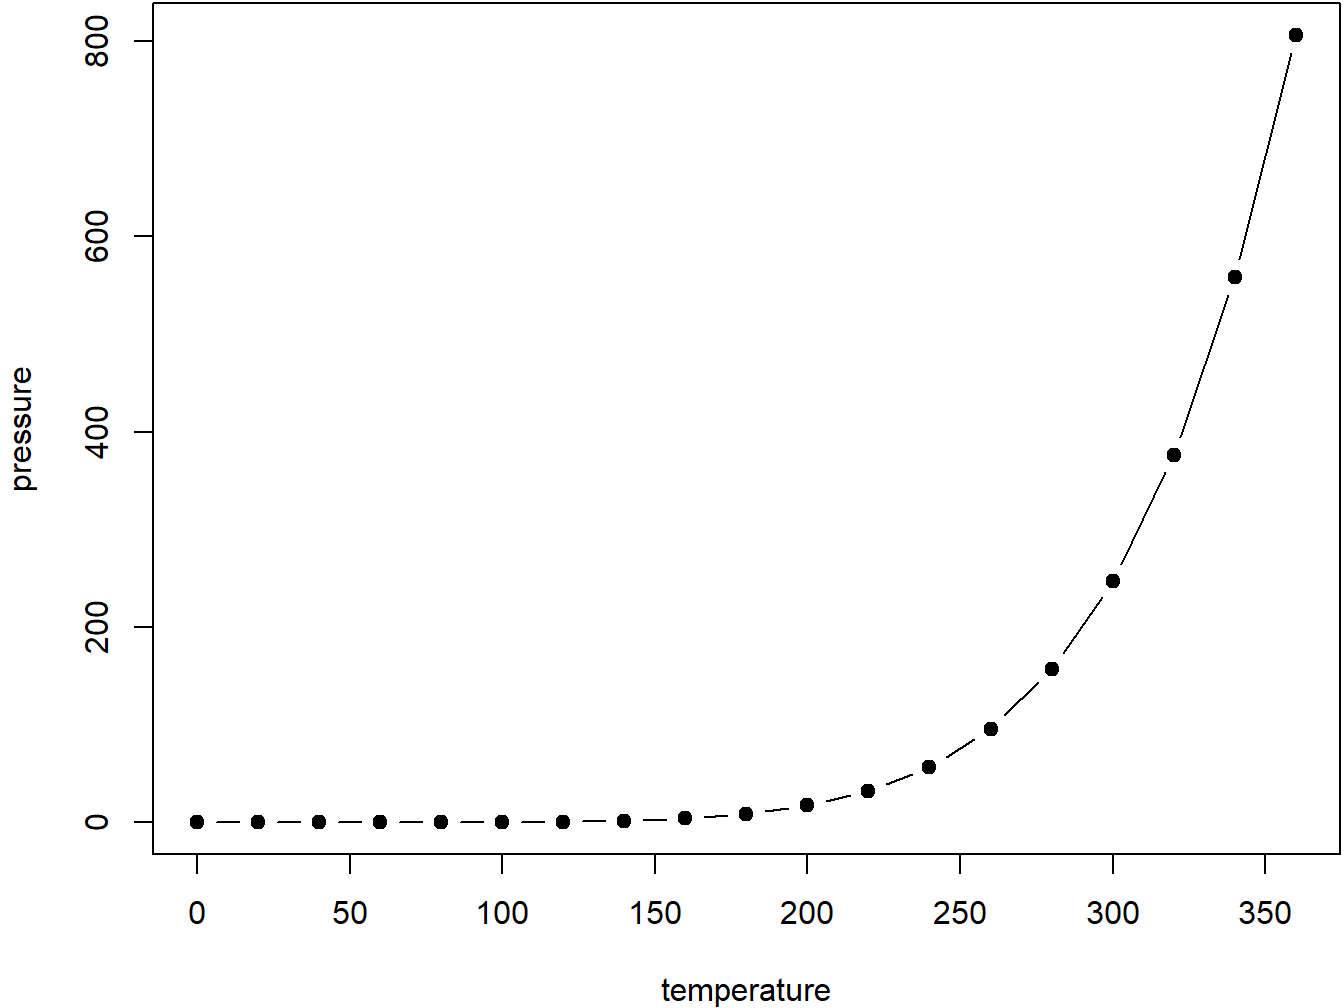
\includegraphics[width=0.8\linewidth]{qgnotes_files/figure-latex/nice-fig-1} 

}

\caption{Here is a nice figure!}\label{fig:nice-fig}
\end{figure}

Reference a figure by its code chunk label with the \texttt{fig:} prefix, e.g., see Figure \ref{fig:nice-fig}. Similarly, you can reference tables generated from \texttt{knitr::kable()}, e.g., see Table \ref{tab:nice-tab}.

\begin{Shaded}
\begin{Highlighting}[]
\NormalTok{knitr}\SpecialCharTok{::}\FunctionTok{kable}\NormalTok{(}
  \FunctionTok{head}\NormalTok{(iris, }\DecValTok{20}\NormalTok{), }\AttributeTok{caption =} \StringTok{\textquotesingle{}Here is a nice table!\textquotesingle{}}\NormalTok{,}
  \AttributeTok{booktabs =} \ConstantTok{TRUE}
\NormalTok{)}
\end{Highlighting}
\end{Shaded}

\begin{table}

\caption{\label{tab:nice-tab}Here is a nice table!}
\centering
\begin{tabular}[t]{rrrrl}
\toprule
Sepal.Length & Sepal.Width & Petal.Length & Petal.Width & Species\\
\midrule
5.1 & 3.5 & 1.4 & 0.2 & setosa\\
4.9 & 3.0 & 1.4 & 0.2 & setosa\\
4.7 & 3.2 & 1.3 & 0.2 & setosa\\
4.6 & 3.1 & 1.5 & 0.2 & setosa\\
5.0 & 3.6 & 1.4 & 0.2 & setosa\\
\addlinespace
5.4 & 3.9 & 1.7 & 0.4 & setosa\\
4.6 & 3.4 & 1.4 & 0.3 & setosa\\
5.0 & 3.4 & 1.5 & 0.2 & setosa\\
4.4 & 2.9 & 1.4 & 0.2 & setosa\\
4.9 & 3.1 & 1.5 & 0.1 & setosa\\
\addlinespace
5.4 & 3.7 & 1.5 & 0.2 & setosa\\
4.8 & 3.4 & 1.6 & 0.2 & setosa\\
4.8 & 3.0 & 1.4 & 0.1 & setosa\\
4.3 & 3.0 & 1.1 & 0.1 & setosa\\
5.8 & 4.0 & 1.2 & 0.2 & setosa\\
\addlinespace
5.7 & 4.4 & 1.5 & 0.4 & setosa\\
5.4 & 3.9 & 1.3 & 0.4 & setosa\\
5.1 & 3.5 & 1.4 & 0.3 & setosa\\
5.7 & 3.8 & 1.7 & 0.3 & setosa\\
5.1 & 3.8 & 1.5 & 0.3 & setosa\\
\bottomrule
\end{tabular}
\end{table}

You can write citations, too. For example, we are using the \textbf{bookdown} package \citep{R-bookdown} in this sample book, which was built on top of R Markdown and \textbf{knitr} \citep{xie2015}.

\hypertarget{quantitative-genetics}{%
\chapter{Quantitative Genetics}\label{quantitative-genetics}}

This section introduces the basic concepts in quantitative genetics such as:

\begin{itemize}
\tightlist
\item
  Genetic value and variance for a quantitative trait
\item
  Genetic parameters (heritability, genetic variance and correlation)
\item
  Difference between genetic values and breeding values
\item
  Infinitesimal model
\end{itemize}

These concepts are relevant for a range of genetic and statistical analyses of complex traits and diseases in animal and plant populations, including:

\begin{itemize}
\tightlist
\item
  Estimating the effect of single locus (or marker) for gene discovery
\item
  Estimating the effect of multiple loci (or markers) for genomic prediction
\item
  Estimating the heritability of a trait (the part of its variability due to genetics)
\item
  Estimating breeding values by pedigree or genomic information
\item
  Selection of breeding individuals based on estimated breeding values
\item
  Prediction of selection response based on estimated heritability (breeder's equation)
\end{itemize}

In the appendix, further details about the quantative genetic models are presented, but these may be outside the scope of this BSc course.

Quantitative genetics, also referred to as the genetics of complex traits, is the study of quantitative traits. Quantitative genetics is based on models in which many genes influence the trait, and in which non-genetic factors may also be important. Quantitative traits such as size, obesity or longevity vary greatly among individuals. Their phenotypes are continuously distributed phenotypes and do not show simple Mendelian inheritance (i.e., their phenotypes are distributed in discrete categories determined by one or a few genes). The quantitative genetics framework can also be used to analyze discrete traits like litter size (which consist of discrete counts like 0, 1, 2, 3, \ldots) or binary traits like survival to adulthood (which consist of 0 or 1, `dead' or `alive', etc.), provided that they have a polygenic basis (i.e., they are determined by many genes). The quantitative genetics approach has diverse applications: it is fundamental to an understanding of variation and covariation among relatives in natural and managed populations; it is also used as basis for selective breeding methods in animal and plant populations (\url{https://doi.org/10.1098/rstb.2009.0203}).

\hypertarget{infinitesimal-model}{%
\section{Infinitesimal model}\label{infinitesimal-model}}

The infinitesimal model, also known as the polygenic model, is a widely used genetic model in quantitative genetics. Originally developed in 1918 by Ronald Fisher, it is based on the idea that variation in a quantitative trait is influenced by an infinitely large number of genes, each of which makes an infinitely small (infinitesimal) contribution to the phenotype, as well as by environmental (non-genetic) factors. In the most basic model the phenotype (P) is the sum of genetic effects (G), and environmental effect (E):

\begin{align}
P = G + E
\end{align}

The genetic effect (G) in the model can be split into additive effects (A), dominance effects (D), and epistatic effects (I) such that the expanded infinitesimal model becomes:

\begin{align}
P = A + D + I + E
\end{align}

The genetic effect may also depend on the environment in which they are expressed (e.g., in plants a drought-tolerance gene may have a favorable effect on grain yield under water-limited conditions, but may be useless under irrigation). Therefore we may consider an extended version of the infinitesimal model where the phenotype (P) is the sum of genetic effects (G), environmental effect (E), and genotype-environment interaction effects (G×E):

\begin{align}
P = G + E + GxE
\end{align}

In practice, the genotype-environment interaction effect can be important for the phenotype of individuals, but for the sake of simplicity we will ignore them in the remainder of this section. Therefore, hereafter, we will assume that genotypic effects are not impacted by environmental factors.

\hypertarget{genetic-effects-genetic-values-and-breeding-values}{%
\subsection{Genetic effects, genetic values and breeding values}\label{genetic-effects-genetic-values-and-breeding-values}}

The genetic effect (G) in the model can include additive effects (A), dominance effects (D), and epistatic effects (I). Additive effects are the summed effects of individual alleles. Dominance effects are interactions between alleles within loci. Epistatic effect are interactions between alleles in different loci and can therefore only occur if two or more loci affect the trait.

Consider an individual that is diploid, like most animals and plants like maize, soybean, barley (i.e., they carry two copies of every genes, except in their sexual chromosomes). Assume that one locus in its genome exists under two possible alleles: A1 and A2, with respective allele effects +1 and -1. How do the individual's alleles combine into a genotype? They may combine additively, so that the value of a genotype (the combination of two alleles genotype) is simply the sum of allele effects, but this is only a very special case! If genetic effects are entirely additive, then the value of each possible genotype is the sum of their respective allele effects, i.e., -2 if the individual is A2A2, 0 if it is A2A1 (or A1A2), and +2 if it is A1A1. Generally, the value of each genotype will depend on the combination of alleles within one locus (G = A + D) or across multiple loci (G = A + D + I). For example, in presence of dominance, the value of each possible genotype may be -2 if the individual is A2A2, +1 if it is A2A1 (or A1A2), and +2 if it is A1A1.

\hypertarget{additive-effects}{%
\subsubsection{Additive Effects}\label{additive-effects}}

Additive effects are the summed effects of average allele effects. Quite confusingly, additive effects depend on the population, because average allele effects depend on the frequency of genotypes in the population! For example, assume that genotypes have values -2 (A2A2), +1 (A2A1) and +2 (A1A1). In a population consisting of 25\% A2A2, 50\% A2A1 and 25\% A1A1, you would expect the A1 allele in a A1A2 genotype 2/3 of the time, and you would expect the A1 allele in a A1A1 genotype 1/3 of the time. In another population consisting of 90\% A2A2, 18\% A2A1 and 1\% A1A1, you would expect the A1 allele in a A1A2 genotype about 95\% of the time, and in a A1A1 genotype only about 5\% of the time. As a result, the effect of the A1 allele, averaged over genotypes, will not be the same, from one population to another.
The concept of additive genetic effects and average allele effects is fundamental to quantitative genetics. However, it is one of is most confusing, precisely because of the dependance of allele effects on genotype frequencies.

\hypertarget{dominance-effects}{%
\subsubsection{Dominance Effects}\label{dominance-effects}}

Dominance genetic effects are the interactions among alleles at a given locus. This is an effect that is extra to the sum of the additive allele effects. Each genotype has its own dominance effect, denoted by \(\delta_{ij}\), for the specific combination of alleles i and j, (e.g., \(\delta_{A_{1}A_{2}}\)), and each of them are non-zero quantities. Using the previous example, the additive and dominance effects would give \ldots..to be completed

\hypertarget{epistatic-genetic-effects}{%
\subsubsection{Epistatic Genetic Effects}\label{epistatic-genetic-effects}}

Epistatic genetic effects encompass all possible interactions among the loci impacting the trait, whenever there is more than one such loci. This includes all two-way interactions (e.g., interactions between loci A and B, A and C), three-way interactions (e.g., joint interaction among A, B and C), etc. Epistasis can be decomposed, so it includes interactions between additive effects at different loci, interactions between additive effects at one locus with dominance effects at a second locus, and interactions between dominance effects at different loci.

\hypertarget{genetic-value-versus-breeding-value}{%
\subsubsection{Genetic value versus Breeding value}\label{genetic-value-versus-breeding-value}}

For selective breeding purposes additive genetic effects are of primary interest. This is because additive effects are generally the largest of the genetic effects, and the allelic effects are passed directly to offspring while the other genetic effects are not transmitted to the progeny, and are generally smaller in magnitude. The sum of the additive effects of all loci on a quantitative trait is known as the true breeding value.

\begin{itemize}
\item
  Breeding value = the value of genes to progeny (additive effects only)
\item
  Genetic value = the value of genes to self (which includes additive, dominance and epistatic effects)
\end{itemize}

The difference between genetic value and breeding value is largely largely dominance deviation. This is because an individual can express dominance deviation (e.g.~an A1A2 heterozygote). However, an individual cannot pass on dominance deviation to its progeny as it only transmits one allele (e.g., an A1A2 heterozygote will either transmit a A1 gamete or an A2 gamete to one of its progeny, but not both!)
With fully inbred lines, offspring have the same genotype as their parent, and hence the entire parental genotypic value G is passed along. Hence, favorable interactions between alleles are not lost by randomization under random mating but rather passed along.
When offspring are generated by crossing (or random mating), each parent contributes a single allele at each locus to its offspring, and hence only passes along a part of its genotypic value. This part is determined by the average effect of the allele. However, any favorable interaction between alleles is not passed along to their offspring.

\hypertarget{infinite-number-of-loci-each-with-small-effect-on-the-phenotype}{%
\subsection{Infinite number of loci each with small effect on the phenotype}\label{infinite-number-of-loci-each-with-small-effect-on-the-phenotype}}

Quantitative traits do not behave according to simple Mendelian inheritance laws. More specifically, their inheritance cannot be explained by the genetic segregation of one or a few genes. Even though Mendelian inheritance laws accurately depict the segregation of genotypes in a population, they are not tractable with the large number of genes which typically affect quantitative traits. To better understand the infinitesimal model assume Mendelian inheritance to occur at every locus in the genome. Let's say there are 30,000 gene loci in the genome. The number of alleles at each locus varies from 2 to 30 or more. If we assume that there are only two alleles (3 possible genotypes) per locus, and gene loci segregate independently, then the number of possible genotypes (considering all loci simultaneously) would be \(3^{30000}\) which is large enough to give the illusion of an infinite number of loci. Furthermore each of these loci could contribute additive and dominance effects in addition to interaction effects.

\hypertarget{distribution-of-genetic-and-phenotypic-values-in-single-locus-model}{%
\subsubsection{Distribution of genetic and phenotypic values in single locus model}\label{distribution-of-genetic-and-phenotypic-values-in-single-locus-model}}

First we will consider how to model the genetic basis of a quantitative trait when a single locus affects the trait of interest. We call this a single-locus model. The distribution of the genetic values for a set of individuals will be discrete. The frequency of the genetic values depend on genotype frequencies, which in turn depend on allele frequencies of \(A_1\) and \(A_2\). The phenotype is however also influenced by the environment. If we assume that the environmental effects are normally distributed (e.g.~\(\N(0,\sigma^2=1)\)) then we can observe that the phenotype distribution is infact normally distributed.

\hypertarget{distribution-of-genetic-and-phenotypic-values-in-multiple-loci-model}{%
\subsubsection{Distribution of genetic and phenotypic values in multiple loci model}\label{distribution-of-genetic-and-phenotypic-values-in-multiple-loci-model}}

Now we will consider a multiple-locus model. When several loci are causal (i.e., they have an effect on a certain trait), then we talk about a \textbf{polygenic model}. Letting the number of causal loci tend to infinity, the resulting model is called an \textbf{infinitesimal model}. From a statistical point of view, the breeding values in an infinitesimal model are considered random with a known distribution. Due to the central limit theorem, this distribution tends to a normal distribution, because of the infinitely large number of causal loci. The central limit theorem says that the distribution of any sum of a large number of very small effects converges to a normal distribution. In our case where a given trait of interest is thought to be influenced by a large number of genetic loci each having a small effect, the sum of the breeding values of all loci together can be approximated by a normal distribution. The histograms below show a better approximation to the normal distribution for breeding values (summed allele effects at causal loci), as the number of causal loci increases. In practice, 100 independently segregating causal loci may be large enough, so that the infinitesimal model (and the normal approximation is genomic models) is accurate enough for predictions.

\begin{figure}
\centering
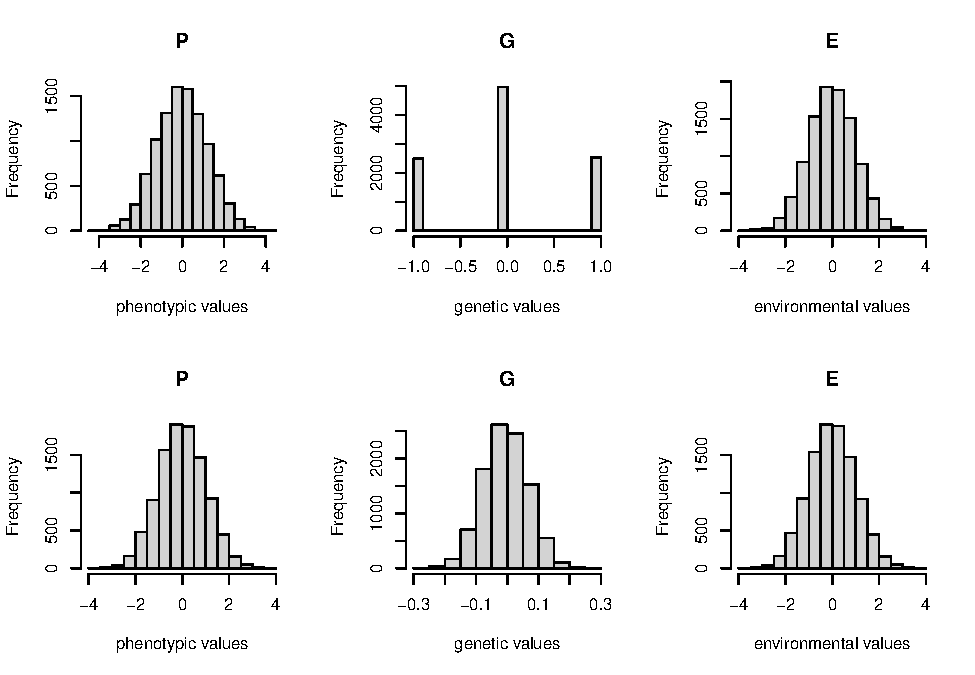
\includegraphics{qgnotes_files/figure-latex/unnamed-chunk-3-1.pdf}
\caption{\label{fig:unnamed-chunk-3}Distribution of genetic and phenotypic values for a quantitative trait influenced by a single locus model (top panel) or multiple loci (bottom panel)}
\end{figure}

\hypertarget{genetic-parameters}{%
\subsection{Genetic parameters}\label{genetic-parameters}}

Fisher (1918) and Wright (1921) have introduced fundamental statistical methods in quantitative genetics:

\begin{itemize}
\tightlist
\item
  analysis of variance: the partition of phenotypic variation into heritable (A) and non-heritable components (D, I and E).
\item
  resemblance among relatives: the estimations of the proportion of loci shared by relatives under the infinitesimal model.
\end{itemize}

\hypertarget{genetic-variance}{%
\subsubsection{Genetic variance:}\label{genetic-variance}}

In the model proposed by Fisher (1918), Cockerham (1954) and Kempthorne (1954), covariance among relatives is described in terms of the additive genetic variance \(V_{A}\) (variance of additive genetic effects, or breeding values), dominance variance \(V_{D}\) (variance of interaction effects between alleles in the same locus), and epistatic variance \(V_{AA}\), \(V_{AD}\), \(V_{DD}\), \ldots. (variance of interaction effects -- additive and/or dominance effects -- among loci) (Falconer \& Mackay 1996; Lynch \& Walsh 1998). These partitions are not dependent on numbers of genes or how they interact, but in practice the model is manageable only when the effects are independent from each other, requiring many important assumptions. These include random mating, and hence Hardy-Weinberg equilibrium (i.e.~no inbred individuals), linkage equilibrium (independent segregation of loci, which requires many generations to achieve for tightly linked genes) and no selection.

\begin{align}
V_{P} &= V_{G} + V_{E} \notag \\
      &= V_{A} + V_{D} + V_{I} + V_{E}
\end{align}

\begin{align}
\sigma^2_{P} &= \sigma^2_{G} + \sigma^2_{E}  \notag \\
             &= \sigma^2_{A} + \sigma^2_{D} + \sigma^2_{I} + \sigma^2_{E}
\end{align}

Many more terms may be included, such as maternal genetic effects, and genotype × environment interaction. The model has unlimited opportunities for complexity. This is a strength, in that it is all-accommodating, and a weakness, in that datasets may allow to partition only a few components. In practice, assumptions must be made to reduce the complexity of the resemblance among relatives. Usually, the resemblance among relatives is assumed to depend only on additive genetic variance \(V_{A}\) and dominance variance \(V_{D}\), so that the following sources of covariation are neglected:

\begin{itemize}
\tightlist
\item
  Epistatic variance (interaction effects among loci are small compared to additive and dominance effects)
\item
  Environmental variance (effects of \textbf{shared environments} are assumed to be small enough)
\end{itemize}

\hypertarget{heritability}{%
\subsubsection{Heritability:}\label{heritability}}

The models and summary statistics defined by Fisher and Wright have remained at the heart of quantitative genetics, not least because they provide ways to make predictions of important quantities, such as

\begin{itemize}
\tightlist
\item
  Breeding value (\(A\)), the expected performance of of an individual's offspring
\item
  Broad-sense heritability, the ratio of total genetic variance V\_G to the overall phenotypic variance \(V_{P}\):
\end{itemize}

\begin{align}
H^2 &= V_{G}/V_P \notag \\
    &= (V_{A} + V_{D} + V_{I})/V_P  \notag \\
H^2 &= \sigma^2_{G}/\sigma^2_P  \notag \\
    &= (\sigma^2_{A} + \sigma^2_{D} + \sigma^2_{I})/\sigma^2_P  \notag 
\end{align}

\begin{itemize}
\tightlist
\item
  Narrow-sense heritability, the ratio of additive genetic variance \(V_{A}\) to the overall phenotypic variance \(V_{P}\):
\end{itemize}

\begin{align}
h^2 &= V_{A}/V_P  \notag \\
h^2 &= \sigma^2_{A}/\sigma^2_P
\end{align}

\begin{itemize}
\tightlist
\item
  The response to artificial or natural selection, the increase (or decrease) of genetic values due to selection of individuals, over generations
\end{itemize}

In view of the assumed complexity of the underlying gene action, involving many loci with unknown effects and interactions, much quantitative genetic analysis has, unashamedly, been at a level of the `black box'.

\hypertarget{genetic-correlation}{%
\subsubsection{Genetic correlation:}\label{genetic-correlation}}

In a general quantitative genetic model, in which, for each individual, two traits (\(P_1\) and \(P_2\)) are are each defined as the sum of a genetic value (\(G_1\) and \(G_2\)) and a environmental value (\(E_1\) and \(E_2\)):
\begin{align}
P_1 = G_1 + E_1 \\
P_2 = G_2 + E_2
\end{align}

The phenotypic correlation (\(\rho_{P_{12}}\)) between the traits is defined as:

\[\rho_{P_{12}}=\frac{\sigma_{P_{12}}}{\sqrt{\sigma_{P_{1}}^2 \sigma_{P_{2}}^2}}\]

where \(\sigma_{P_{12}}\) is the phenotypic covariance and \(\sigma_{P_{1}}^2\) and \(\sigma_{P_{2}}^2\) are the variances of the phenotypic values for the two traits in the population.
The genetic correlation (\(\rho_{G_{12}}\)) of the traits is defined as:

\[\rho_{G_{12}}=\frac{\sigma_{G_{12}}}{\sqrt{\sigma_{G_{1}}^2 \sigma_{G_{2}}^2}}\]

where \(\sigma_{G_{12}}\) is the genetic covariance and \(\sigma_{G_{1}}^2\) and \(\sigma_{G_{2}}^2\) are the variances of the genetic values for the two traits in the population.

\hypertarget{basic-questions-remain}{%
\subsection{Basic questions remain}\label{basic-questions-remain}}

On the premise that many genes and environmental factors interact to impact the trait, it will be difficult to determine the action of individual causal genes. Many basic questions remain: What do the genes do; how do they interact; on what traits does natural selection act; why is there so much genetic variation; and can we expect continued genetic improvement in selection programmes? Ultimately, we want to know at the molecular level not just which genes are involved, whether structural or regulatory, but what specific mutation (nucleotide substitution, deletious, copy number variant, etc.) is responsible for genetic effects, and how the causal genes are controlled.

\hypertarget{estimation-of-genetic-parameters}{%
\chapter{Estimation of Genetic Parameters}\label{estimation-of-genetic-parameters}}

This section introduces the basic concepts of estimating genetic parameters such as:

\begin{itemize}
\tightlist
\item
  basic principles of estimating genetic parameters
\item
  use of genetic relationships for estimating genetic parameters
\item
  different methods, data sources and experimental designs for estimating genetic parameters
\item
  importance of estimation of genetic parameters in breeding
\item
  knowing when estimation of genetic parameters may be required
\end{itemize}

The estimation of genetic parameters is an important issue in animal and plant breeding. First of
all, estimating additive genetic and possible non-additive genetic variances contributes
to a better understanding of the genetic mechanism. Secondly, estimates of genetic and
phenotypic variances and covariances are essential for the prediction of breeding values
and for the prediction of the expected genetic response of
selection programmes. Parameters that are of interest are heritability, genetic and
phenotypic correlation and repeatability, and those are computed as functions of the
variance components.

Genetic parameters are estimated using information on phenotypes and genetic relationships
for individuals in the breeding population. Heritability is estimated by comparing individual
phenotypic variation among related individuals in a population. Close (compared to distant) relatives
share more DNA in common and if the trait is under genetic influence they will therefore share
phenotypic similarities. In this section we will illustrate how different phenotypic sources
and genetic relationships are used for estimating genetic parameters.

\hypertarget{genetic-model}{%
\section{Genetic model}\label{genetic-model}}

As introduced previously the phenotype for a quantitative trait is the sum of both genetic and environmental factors. In general the total genetic effect for an individual is the sum of both additive and non-additive effects. However, only the additive genetic effects are passed on to the offspring and therefore have a breeding value. Therefore we only consider the additive genetic model as the basis for estimation of genetic parameters. The model for the phenotype (\(y\)) is:
\begin{align}
            y=\mu+a+e    \notag
\end{align}
where \(\mu\) is the population mean, \(a\) is the additive effect, and \(e\) is the environmental deviation (or residual) not explained by the genetic effects in the model.
We assume that the additive genetic effect, a, and the residual term, e, are normally distributed which means that the observed phenotype is also normally distributed
\begin{align}
a \sim N(0,\sigma^2_{a}), \quad
e \sim N(0,\sigma^2_{e}), \quad
y \sim N( \mu,\sigma^2_{y}) \notag
\end{align}
where \(\sigma^2_{a}\) is additive genetic variance, \(\sigma^2_{e}\) is residual variance, and (\(\sigma^2_{y}\)) is the total phenotypic variance.

\hypertarget{genetic-parameters}{%
\section{Genetic parameters}\label{genetic-parameters}}

Heritability and genetic correlation are the key genetic parameters used in animal and plant breeding. They are defined in terms of the variance component (\(\sigma^2_{a}\) and \(\sigma^2_{e}\)) defined in the previous section.

\textbf{Heritability} estimates the degree of variation in a phenotypic trait in a population that is due to genetic variation between individuals in that population. It measures how much of the variation of a trait can be attributed to variation of genetic factors, as opposed to variation of environmental factors. The narrow sense heritability is the ratio of additive genetic variance (\(\sigma^2_{a}\)) to the overall phenotypic variance (\(\sigma^2_{y}=\sigma^2_{a}+\sigma^2_{e}\)):
\begin{align}
h^2 &= \sigma^2_{a}/(\sigma^2_a+\sigma^2_e)
\end{align}
A heritability of 0 implies that the no genetic effects influence the trait, while a heritability of 1 implies that all of the variation in the trait is explained by the genetic effects. In general the amount of information provided by the phenotype about the breeding value is determined by the narrow sense heritability.

\textbf{Genetic correlation} is the proportion of variance that two traits share due to genetic causes. Genetic correlations are not the same as heritability, as it is about the overlap between the two sets of influences and not their absolute magnitude; two traits could be both highly heritable but not be genetically correlated or have small heritabilities and be completely correlated (as long as the heritabilities are non-zero).
Genetic correlation (\(\rho_a\)) is the genetic covariance between two traits divided by the product of genetic standard deviation for each of the traits:
\begin{align}
\rho_{a_{12}}=\frac{\sigma_{a_{12}}}{\sqrt{\sigma_{a_{1}}^2 \sigma_{a_{2}}^2}}
\end{align}
where \(\sigma_{a_{12}}\) is the genetic covariance and \(\sigma_{a_{1}}^2\) and \(\sigma_{a_{2}}^2\) are the variances of the additive genetic values for the two traits in the population.
A genetic correlation of 0 implies that the genetic effects on one trait are independent of the other, while a correlation of 1 implies that all of the genetic influences on the two traits are identical.
Thus in order to estimate the heritability and genetic correlation we need to estimate the variance component defined above.

\hypertarget{data-required-for-estimating-genetic-parameters}{%
\section{Data required for estimating genetic parameters}\label{data-required-for-estimating-genetic-parameters}}

Information on phenotypes and genetic relationships for individuals in the breeding population
are used to formulate appropriate statistical models for the analysis of the data
and accurate estimation of genetic parameters and breeding values of individuals.

\textbf{Phenotypes} for traits of economic importance need to be recorded accurately and completely. All individuals
within a production unit (herd, flock, ranch, plot) should be recorded. Individuals should not be
selectively recorded. Data includes the dates of events when traits are observed, factors
that could influence an individual's performance, and an identification of contemporaries that
are raised and observed in the same environment under the same management regime.
Observations should be objectively measured, if at all possible.

\textbf{Genetic relationships} for the individuals in the breeding population is required. Genetic relationships can be inferred from a pedigree or alternative alternative from genetic markers. Individuals and their parents need to be uniquely identified in the data. Information about birth dates, breed composition, and genotypes for various markers or QTLs could also be stored. If individuals are not uniquely identified, then genetic change of the population may not be
possible. In aquaculture species, for example, individual identification may not be feasible,
but family identification (father and mother) may be known.

Furthermore knowledge and understanding of the production system is
important for designing optimum selection and mating strategies. For dairy cattle key elements are the
gestation length and the age at first breeding. The number of offspring per female per
gestation will influence family structure. The use of artificial insemination and/or embryo
transfer could be important. Other management practices are also useful to know.

Prior information about the traits is useful. Read the literature. Most likely other researchers or
breeders have already made analyses of the same species and traits. Their models could be useful
starting points for further analyses. Their parameter estimates could predict the kinds of
results that might be found. The idea is to avoid the pitfalls and problems that other
researchers have already encountered. Be aware of new kinds of analyses of the same data,
that may not involve statistical models.

\hypertarget{statistical-models-and-variance-components}{%
\section{Statistical models and variance components}\label{statistical-models-and-variance-components}}

For estimating genetic parameters we need to specify a model that describes the genetic and non-genetic factors that may affect the trait phenotypes. Often the non-genetic factors are referred to as systematic effect
such as age, parity, litter size, days open, sex, herd, year, season, management, etc.

\begin{align}
            \text{mean}=\text{mean} + \text{systematic effect} + \text{genetic effect}  + residual   \notag
\end{align}

In this, we make a distinction between fixed effects, that determine the level (expected means) of observations, and
random effects that determine variance. A model at least exists of one fixed (mean)
and one random effect (residual error variance). If observations also are influenced by a
genetic contribution of the individuals, then a genetic variance component exists as well. In
that situation, we have two components contributing to the total variance of the
observations: a genetic and a residual variance component.

A statistical model is usually specified as a mathematical relationship between one or more random variables and other non-random variables. In quantitative genetics it is often based on the additive genetic model specified above with inclusion of additional factors that may affect the trait of interest:

\begin{align}
            y=\mu + \text{...systematic effect....} + a + e  \notag
\end{align}

where \(\mu\) is the population mean, \(a\) is the additive effect, and \(e\) is the environmental deviation (or residual) not explained by the systematic effects and the genetic effects in the model. We assume that the additive genetic effect, a, and the residual term, e, are normally distributed such that \(a \sim N(0,\sigma^2_{a})\) and \(e \sim N(0,\sigma^2_{e})\). The goal of the statistical analysis is to derive estimates for the variance components that is the additive genetic variance \(\sigma^2_{a}\), and the residual variance \(\sigma^2_{e}\) the residual variance.

The statistical model is a formal representation of our quantitative genetic theory, but it is important to realize that all models are simple approximations to how factors influence a trait. The goal of the statistical analysis is to find the best practical model that explains the most variation in the data. Statistical knowledge is required. The methods used for estimating genetic parameters is based on statistical concepts such as random variables, multivariate normal theory and linear (mixed) models. These concepts and their use will be explained in the following sections.

\hypertarget{methods-for-estimation-of-genetic-parameters}{%
\chapter{Methods for estimation of genetic parameters}\label{methods-for-estimation-of-genetic-parameters}}

In general estimation of heritability and genetic correlation is based on methods that determine resemblance
between genetically related individuals. Here we will present three methods for estimating heritability, parent-offspring regression, analysis of variance (ANOVA) for family data (e.g.~halfsib/fullsib families) and restricted maximum likelihood (REML) analysis for general pedigree.

\hypertarget{estimating-heritability-using-parent---offspring-regression}{%
\section{Estimating heritability using parent - offspring regression}\label{estimating-heritability-using-parent---offspring-regression}}

The simplest method for estimation genetic parameters is based on regression analysis.
Heritability may be estimated by comparing phenotypes for traits recorded in parent and offspring. Parent-offspring regression compares trait values in parents (\(y_p\)) to trait values in their offspring (\(y_o\)). Estimation of heritability is based on a linear regression model:
\begin{align}
            y_o &= y_p b_{o|p}+e_o. \notag \\
\end{align}
The slope of the regression line (\(b_{o|p}\)) approximates the heritability of the trait when offspring values are regressed against the average trait in the parents. If only one parent's value is used then heritability is twice the slope. In other words the expected value of the regression line is \(b_{o|p} = 0.5h^2\) (or h2 when
regression is on mid-parent mean).

To better understand this relationship consider a situation
where we have collected phenotypes on a number of father-offspring families.
From standard regression theory the slope can be determined as:
\begin{align}
            b_{o|f} &= \frac{Cov(y_f,y_o)}{Var(y_o)} \notag \\
\end{align}
where \(Cov(y_f,y_o)\) is the covariance between the phenotypes of the father and the offspring and \(Var(y_o)\) is the variance of the offspring phenotypes.

The phenotypes for the father (\(y_f\)) and the offspring (\(y_o\)) can be expressed as:
\begin{align}
            y_f &= \mu+a_f+e_f \notag \\
            y_o &= \mu+0.5a_m+0.5a_f+a_{mendelian}+e_o \notag
\end{align}
where \(\mu\) is the population mean, \(a_m\) and \(a_f\) are the additive genetic effect for the mother and the father, a\_\{mendelian\} is the mendelian deviation in the offspring, and \(e_f\) and \(e_o\) are the residual effect for the father and the offspring.

The offspring get half of the genes from each parent and therefore the breeding value for the offspring is the average of the parents' breeding values plus the Mendelian deviation:
\begin{align}
        a_{\text{offspring}}=\frac{1}{2}a_{\text{father}}+\frac{1}{2}a_{\text{mother}}+a_{\text{mendelian}} \notag  
\end{align}
(a = additive genetic value = breeding value)
The term \(a_{mendelian}\) is necessary, because two fullsibs \(i\) and \(j\) both having parents \(father\) and \(mother\) receive different random samples of the set of parental alleles. Hence the breeding values \(a_i\) and \(a_j\) of halfsibs \(i\) and \(j\) are not going to be the same.
Furthermore we assume that the breeding values are normally distributed:
\begin{align}
a_{father} \sim N(0,\sigma^2_{a}) \notag \\
a_{mother} \sim N(0,\sigma^2_{a}) \notag \\
a_{mendelian} \sim N(0,0.5\sigma^2_{a}) \notag \\
\end{align}

Therefor an expression for the covariance between the phenotypes of the parent and the offspring can be derived as:\\
\begin{align}
            Cov(y_f,y_o) &= Cov(a_f+e_f,0.5a_m+0.5a_f+a_{mendelian}+e_o) \notag \\
                         &= Cov(a_f,0.5a_f) \notag \\
                         &= 0.5Cov(a_f,a_f) \notag \\
                         &= 0.5\sigma_a^2 \notag 
\end{align}
and similar for the variance variance of the offspring phenotypes:\\
\begin{align}
            Var(y_o) &= Var(0.5a_m+0.5a_f+0.5a_{mendelian}+e_o) \notag \\
                     &= Var(0.5a_m) + Var(0.5a_f) + Var(a_{mendelian}) + Var(e_o) \notag \\
                     &= 0.25Var(a_m) + 0.25Var(a_f) + Var(a_{mendelian}) + Var(e_o) \notag \\
                     &= 0.25\sigma_a^2 + 0.25\sigma_a^2 + 0.5\sigma_a^2 + \sigma_e^2 \notag \\
                     &= \sigma_a^2 + \sigma_e^2 \notag
\end{align}
Therefore the expected value of the regression coefficient for a father-offspring analysis is:
\begin{align}
            b_{o|f} &= \frac{0.5\sigma_a^2}{\sigma_a^2 + \sigma_e^2} \notag \\
                    &= 0.5\frac{\sigma_a^2}{\sigma_a^2 + \sigma_e^2} \notag \\
                    &= 0.5h^2 \notag \\
            h^2     &= 2b_{o|f}\notag
\end{align}

Similar relationships can be derived for other types of parent-offspring regression analysis (mother-offspring and mid- parent-offspring). The heritability can be estimated from the regression coefficient based on:\\
\begin{align}
    h^2 &= 2b_{o|m} \quad \text{(mother-offspring regression)} \notag \\
    h^2 &= 2b_{o|f} \quad \text{(father-offspring regression)} \notag \\
    h^2 &=  b_{o|mf} \quad \text{(mean parent-offspring regression)} \notag
\end{align}

Offspring-parent regression is not often used in practice.
It requires data on 2 generations, and uses only this data. It is based on the genetic relationship between parent and offspring which equals 0.5 (i.e.~offspring get half of the genes form its parent), but it is not possible to
utilize genetic relationships among parents. However, the method is robust against
selection of parents.

\hypertarget{estimating-heritability-using-anova-for-family-data}{%
\section{Estimating heritability using ANOVA for family data}\label{estimating-heritability-using-anova-for-family-data}}

Genetic parameters have been estimated for many years using analysis of variance
(ANOVA). This method require that individuals can be assigned to groups with the
same degree of genetic relationship for all members. Family structures considered most often
are paternal half-sib groups or full-sib groups. In the case of paternal half-sib group all
offspring of one sire are treated as one group and offspring of different sires are
allocated to different groups.

Estimation of heritability using ANOVA is based on a linear model.
Consider a situation where we have phenotypic observation for multiple offspring for a number of families (halfsib or fullsib).
A simple linear model for the phenotypic observation for the jth offspring in the ith famility include the population mean (\(\mu\)) and a family effect (\(f_i\)):
\begin{align}
 y_{ij} &= \mu + f_i + e_{ij}
\end{align}

Assume n observations, with \(n_f\) families, with \(n_o\) is the number of offspring per family.

The total sum of squares (SST) is the sum of each of the observations squared:
\begin{align}
 SST &= \sum_{i=1}^{n_f}\sum_{j=1}^{n_o} {y}_{ij}^2
\end{align}

where \(y_{ij}\) is an observation on the jth offspring in the ith family.

The mean sum of squares (SSM) is n times the mean squared:
\begin{align}
 SSM &= n\bar{y}_{..}^2
\end{align}

The model sum of squares (SSA) due to a particular factor (e.g.~the family effect) is therefore the sum over all observations of the estimated (family) effect in each observation squared (in balanced data this
is the difference between the family group mean and the overall mean):
\begin{align}
 SSA &= \sum_{i=1}^{n_f} (\bar{y}_{i.}-\bar{y}_{-.})^2
\end{align}
Notice that the sum of squares for the main effect (SSA) is the sum of all the squared
estimates of \(f_i\), because in a balanced data set the estimate of \(f_i\) is equal to (\(y_{i}.-y_{..}\)). In a
balanced data, it is rather simple to determine the expectations for each sum of squares,
because the number of observations per class of f is constant (\(n_o\)).

The residual sum of squares (SSE) due to the residual (error) is the sum over all
observations of the residual effect in each observation squared (this is the
difference between the observation and its group mean):

\begin{align}
 SSE &= \sum_{i=1}^{n_f}\sum_{j=1}^{n_o} {y}_{ij}^2
\end{align}

The total sum of squares can be expressed as a sum of the components described above:\\
\begin{align}
 SST &= SSM + SSA + SSE
\end{align}

In balanced data, it is rather simple to estimate variance components, by setting
the ``Mean Squares'' equal to their expectations. Those expectations are linear functions
of the variance components and is derived based on statistical theory (Expected value
of a sum of squares).
In this simple model we can calculate estimate of the residual variance components (\(\hat{\sigma}^2_{e}\)) as:
\begin{align}
 \hat{\sigma}^2_{e} &= SSE/(n-n_f)
\end{align}
and and estimate of the family variance (\(\hat{\sigma}^2_{f}\)) as:
\begin{align}
 \hat{\sigma}^2_{f} &= (SSA/(n_f-1) - \hat{\sigma}^2_{e})/n_o
\end{align}

Calculating the variance between groups, involves partitioning the sum of squared
observations (SS) due to different sources of variation in the model of analysis, groups
of relatives being one of them, and equating the corresponding mean squares. Mean
squares are derived as the SS divided by the associated degrees of freedom, to their
expectations.

Using ANOVA, the covariance among members of a family or group of relatives is
usually determined as the variance component between groups. For example, in case of
a half-sib family model, the variance between half-sib families \(\sigma_{s}^2\)
and variance within half-sib families \(\sigma_{e}^2\).
As shown earlier, the half-sib family variance \(\sigma_{s}^2=0.25\sigma_{a}^2\)
while the variance within half-sib families is \(0.75\sigma_{a}^2+\sigma_{e}^2\)

Fullsib families
\begin{align}
            y_m &= \mu+a_m+e_m \notag \\
            y_f &= \mu+a_f+e_f \notag \\
            y_{o1} &= \mu+0.5a_m+0.5a_f+0.5a_{mendelian_1}+e_{o1} \notag \\
            y_{o2} &= \mu+0.5a_m+0.5a_f+0.5a_{mendelian_2}+e_{o2} \notag
\end{align}
\begin{align}
            Cov(y_{o1},y_{o2}) &= Cov(0.5a_m+0.5a_f+a_{mendelian1}+e_{o1},0.5a_m+0.5a_f+a_{mendelian2}+e_{o2}) \notag \\
                         &= Cov(0.5a_f,0.5a_f) + Cov(0.5a_m,0.5a_m) \notag \\
                         &= 0.25Cov(a_f,a_f)+0.25Cov(a_m,a_m) \notag \\
                         &= 0.25\sigma_a^2 +0.25\sigma_a^2 \notag \\
                         &= 0.5\sigma_a^2 \notag
\end{align}
Halfsib families
\begin{align}
            y_{m1} &= \mu+a_{m1}+e_{m1} \notag \\
            y_{m2} &= \mu+a_{m2}+e_{m2} \notag \\
            y_f &= \mu+a_f+e_f \notag \\
            y_{o1} &= \mu+0.5a_{m1}+0.5a_f+0.5a_{mendelian1}+e_{o1} \notag \\
            y_{o2} &= \mu+0.5a_{m2}+0.5a_f+0.5a_{mendelian2}+e_{o2} \notag
\end{align}
\begin{align}
            Cov(y_{o1},y_{o2}) &= Cov(0.5a_{m1}+0.5a_f+a_{mendelian1}+e_{o1},0.5a_{m2}+0.5a_f+a_{mendelian2}+e_{o2}) \notag \\
                         &= Cov(0.5a_f,0.5a_f) + Cov(0.5a_{m1},0.5a_{m2}) \notag \\
                         &= 0.25Cov(a_f,a_f) + 0 \notag \\
                         &= 0.25\sigma_a^2 \notag \\
                         &= 0.25\sigma_a^2 \notag
\end{align}

Therefore the heritability can be estimated from the variance component based on:\\
\begin{align}
    \sigma_{hs}^2 &= 0.25\sigma_a^2 \quad \text{(halfsib families)} \notag \\
    \sigma_{fs}^2 &= 0.5\sigma_a^2 \quad \text{(halfsib families)} \notag \\
    h^2 &= \frac{4\sigma_{hs}^2}{4\sigma_{hs}^2+\sigma_e^2} \quad \text{(halfsib families)} \notag \\
    h^2 &= \frac{2\sigma_{fs}^2}{2\sigma_{fs}^2+\sigma_e^2} \quad \text{(fullsib families)} \notag \\
\end{align}

Data arising from experimental designs used for estimating genetic parameters
are usually not balanced (i.e.~number of offspring varies across families).
Methods analogous to the ANOVA have been developed for unbalanced data.
However REML is nowadays the method of choice for variance component estimation.

The estimation of variance components (within and between family components). If
the variation within families is large relative to differences between families, the trait
must be lowly heritable. Variance components are attributed to specific effects. For
example, the (paternal) half-sib variance is due to differences between sires. The
variance component represents the sire variance, which is a quarter of the additive
genetic variance.

Estimation of variance components is easier to generalise, and this method is generally
used to estimate genetic parameters. The remainder of this chapter will therefore mostly deal with
variance component estimation.

\hypertarget{estimating-heritability-using-restricted-maximum-likelihood}{%
\section{Estimating heritability using Restricted Maximum Likelihood}\label{estimating-heritability-using-restricted-maximum-likelihood}}

Genetic parameters are nowadays estimated using restricted maximum likelihood (REML) or Bayesian methods.
This method allow for estimation of genetic parameters using phenotypic information for individuals from a general pedigree.REML is based on linear mixed model methodology and use a likelyhood approach for estimating genetic parameters.

\hypertarget{linear-mixed-model}{%
\subsection{Linear mixed model:}\label{linear-mixed-model}}

The linear mixed model contains the observation vector for the trait(s) of interest, the
factors that explain how the observations came to be, and a residual effect that includes
everything not explainable.

A matrix formulation of a general model equation is:
\begin{align}
y &= Xb + Za + e \notag
\end{align}

where
\begin{align}
y &: \text{is the vector of observed values of the trait,} \notag \\
b &: \text{is a vector of factors, collectively known as fixed effects,} \notag \\
a &: \text{is a vector of factors known as random effects,} \notag \\
e &: \text{is a vector of residual terms, also random,} \notag \\
X,Z &: \text{are known design matrices that relate the elements of b and a to their corresponding element in y.} \notag 
\end{align}

The \textbf{observation vector} contains elements resulting from measurements, either subjective
or objective, on the experimental units (usually animals) under study. The elements in
the observation vector are random variables that have a multivariate distribution, and if
the form of the distribution is known, then advantage should be taken of that knowledge.
Usually \(y\) is assumed to have a multivariate normal distribution, but that is not always
true. The elements of \(y\) should represent random samples of observations from some defined
population. If the elements are not randomly sampled, then bias in the estimates of b and
\(a\) can occur, which would lead to errors in ranking individuals.

A \textbf{continuous factor} is one that has an infinite-like range of
possible values. For example, if the observation is the distance a rock can be thrown,
then a continuous factor would be the weight of the rock. If the observation is the
rate of growth, then a continuous factor would be the amount of feed eaten.

\textbf{Discrete} factors usually have classes or levels such as age at calving might have four
levels (e.g.~20 to 24 months, 25 to 28 months, 29 to 32 months, and 33 months or
greater). An analysis of milk yields of cows would depend on the age levels of the
cows.

In the traditional ''frequentist'' approach, \textbf{fixed} and \textbf{random} factors need
to be distinguished.

If the number of levels of a factor is small or limited to a fixed number, then that
factor is usually fixed.
If inferences about a factor are going to be limited to that set of levels, and to no
others, then that factor is usually fixed.
If a new sample of observations were made (a new experiment), and the same levels
of a factor are in both samples, then the factor is usually fixed.
If the levels of a factor were determined as a result of selection among possible
available levels, then that factor should probably be a fixed factor.
Regressions of a continuous factor are usually a fixed factor (but not always).

If the number of levels of a factor is large, then that factor can be a
random factor.
If the inferences about a factor are going to be made to an entire population of
conceptual levels, then that factor can be a random factor.
If the levels of a factor are a sample from an infinitely large population, then that
factor is usually random.
If a new sample of observations were made (a new experiment), and the levels were
completely different between the two samples, then the factors if usually random.

\hypertarget{expectation-and-variance-of-variables-in-the-model}{%
\subsubsection*{Expectation and variance of variables in the model:}\label{expectation-and-variance-of-variables-in-the-model}}
\addcontentsline{toc}{subsubsection}{Expectation and variance of variables in the model:}

In the statistical model (specified above) the random effect (\(a\) and \(e\)) and the phenotypes (\(y\)) are considered to be random variables that are assumed to follow a multivariate normal distribution.\\
In general terms the expectations of these random variables are:\\
\begin{align}
E(y) &= E(Xb) + E(Za) + E(e) \notag \\
     &= Xb + 0 + 0 \notag \\
     &= Xb \notag
\end{align}
and the variance-covariance matrices are:
\begin{align}
 Var(a) &= G \notag \\
 Var(e) &= R \notag \\
 Var(y) &= ZGZ' + R = V \notag \\
\end{align}

where \(G\), \(R\) and \(V\) are square matrices of genetic, residual and phenotypic (co)variances among the individuals in the data set. If we assume

\begin{align}
 Var(a) &= G \notag \\
        &= A\sigma_a^2 \notag \\
 Var(e) &= R \notag \\
        &= I\sigma_e^2 \notag \\
 Var(y) &= ZGZ' + R = V \notag \\
        &= A\sigma_a^2 + I\sigma_e^2 \notag
\end{align}

\hypertarget{assumptions-and-limitations-of-the-model}{%
\subsubsection*{Assumptions and limitations of the model:}\label{assumptions-and-limitations-of-the-model}}
\addcontentsline{toc}{subsubsection}{Assumptions and limitations of the model:}

The third part of a model includes items that are not apparent in parts 1 and 2. For
example, information about the manner in which data were sampled or collected. Were
the animals randomly selected or did they have to meet some minimum standards? Did
the data arise from many environments, at random, or were the environments specially
chosen? Examples will follow. A linear model is not complete unless all three parts of the model are present.
Statistical procedures and strategies for data analysis are determined only after a complete
model is in place.

\hypertarget{likelihood-approach-for-estimating-variance-components}{%
\subsection{Likelihood approach for estimating variance components}\label{likelihood-approach-for-estimating-variance-components}}

Restricted Maximum Likelihood is a method that is used to estimate the parameters in the model (i.e.~variance components \(\sigma_{a}^2\) and \(\sigma_{e}^2\)) specified in the linear mixed model above. The general principle used in likelihood methods is to find the set of parameters which maximizes the likelihood of the data.

It is useful to recall that the likelihood (\(L(\theta|{y})\)) is any function of the parameter (\(\theta\)) that is proportional to \(p({y}|\theta)\). Maximizing \(L(\theta|{y})\) leads to obtaining the most likely value of \(\theta\) (\(\hat{\theta}\)) given the data \({y}\). Usually the likelihood is expressed in terms of its logarithm (\(l(\theta|\bf{y})\)) as it makes the algebra easier.

The likelihood of the data for a given linear mixed model can be written as a function;

\begin{equation} 
    l(\matr{V}|\vect{y}, \matr{X}, \bfbeta) 
    \propto
     -\frac{1}{2}\ln|\matr{V}|
     -\frac{1}{2}\ln|\matr{X'V}^{-1}\matr{X}|
     -\frac{1}{2}(\vect{y}-\matr{X}{\bfbeta})'\matr{V}^{-1}(\vect{y}-\matr{X}{\bfbeta})
    \label{eq:reml.likelihood}
\end{equation}

From calculus we know that we can find the maximum of a function by taking the first
derivative and set that equal to zero. Solving that would result in the desired
parameters (assuming that we did not find the minimum, this can be checked using
second derivatives). The first and second derivatives of the likelihood function
are complicated formulas.

There are no simple one-step solutions for estimating the variance components based on REML \citep{LynchWalsh1998}. Instead, we infer the partial derivatives of the likelihoods with respect to the variance components. The solutions to these involve the inverse of the variance-covariance matrix, which themselves includes the variance components, so the variance components estimates are non-linear functions of the variance components. It is therefore necessary to apply iterative methods to obtain the estimates.

From the estimate of the variance components the heritability can easily computed by
\begin{align}
\hat{h}^2 &= \hat{\sigma}^2_{a}/(\hat{\sigma}^2_a+\hat{\sigma}^2_e)
\end{align}
where the ``\(\hat{h}^2\)'' refers to the heritability is an estimate.

\hypertarget{advantages-of-using-reml-for-estimating-genetic-parameters}{%
\subsection{Advantages of using REML for estimating genetic parameters}\label{advantages-of-using-reml-for-estimating-genetic-parameters}}

The REML method was developed by \citet{Patterson1971} as an improvement of the standard Maximum Likelihood (ML). The ML method was originally proposed by \citet{Fisher1922} but was introduced to variance components estimation by \citet{Hartley1967}. ML assumes that fixed effects are known without error which is in most cases false and, as consequence, it produces biased estimates of variance components (usually, the residual variance is biased downward). To solve this problem, REML estimators maximize only the part of the likelihood not depending on the fixed effects,
by assuming that the fixed effects have been, so to speak, fixed. This entails that when comparing multiple models by their REML likelihoods, they must contain the same fixed effects,
and that REML, by itself, does not estimate the fixed effects.

REML does not produce unbiased estimates owing to the inability to return negative values of variance components of many methods to obtain REML estimators, but it is still the method of choice due to the fact that this source of bias is also present in ML estimates \citep{LynchWalsh1998}.

REML requires that y have a multivariate normal distribution
although various authors have indicated that ML or REML estimators may be an
appropriate choice even if normality does not hold (Meyer, 1990).

REML can account for selection when the complete mixed model is used with
all genetic relationships and all data used for selection included (Sorensen and Kennedy,
1984; Van der Werf and De Boer, 1990).

There is obviously an advantage in using (RE)ML methods that are more flexible in
handling animal and plant breeding data on several (overlapping) generations (and possibly
several random effects). However, the use of such methods has a danger in the sense
that we need not to think explicitly anymore about data structure. To estimate, as an
example, additive genetic variance, we need to have a data set that contains a certain
family structure that allows us to separate differences between families from differences
within families. Or in other words, we need to separate genetic and residual variance.
ANOVA methods require more explicit knowledge about such structure, since the data
has to be ordered according to family structures (e.g.~by half sib groups).

Developments in variance component estimation specific to animal and plant breeding have been
closely linked with advances in the genetic evaluation using Best Linear
Unbiased Prediction (BLUP). Early REML applications were generally limited to models
largely equivalent to those in corresponding ANOVA type analysis, considering one
random effect only and estimating genetic variances from paternal half sib covariances
(so-called sire model). Today, heritability can be estimated from general pedigrees and from genomic relatedness estimated from genetic markers. Linear mixed models is also used genetic evaluation schemes,
allowing information on all known relationships between individuals to be incorporated in
the analysis. Linear mixed models can include maternal, permanent environmental, cytoplasmic or
dominance effects or effects at QTL thereby more accurately describe the observed data.
These effects are fitted as additional random effects.

\hypertarget{when-to-estimate-variance-components}{%
\section{When to estimate variance components?}\label{when-to-estimate-variance-components}}

In general, the estimation of variances and covariances has to be based on a sufficient
amount of data. Depending on the data structure and the circumstances during
measuring, estimations can be based on some hundreds (selection experiments) or more
than 10,000 observations (field recorded data). It is obvious that we are not interested in
estimating variance components from every data set. The information in literature is in
many cases even better than estimations based on a small data set. In general, we have
to estimate variance if:
- we are interested in a new trait, from which no parameters are available;
- variances and covariances might have changed over time
- considerable changes have occurred in a population e.g.~due to recent
importations.
Mostly it is assumed that variances and covariances, and especially the ratio of both of
them (like heritability, correlation), are based on particular biological rules, which do
not rapidly change over time. However, it is well known that the genetic variance
changes as consequence of selection. Changes are especially expected in situations with
short generation intervals, high selection intensities or high degrees of inbreeding or in a
situation in which a trait is determined by only a few genes. Secondly, the
circumstances under which measurements are taken can change. If conditions are
getting more uniform over time, the environmental variance decreases, and
consequently the heritability increases. Thirdly, the biological interpretation of a trait
can change as consequence of a changed environment; feed intake under limited
feeding is not the same as feed intake under ad-lib feeding. In conclusion, there are
sufficient reasons for regular estimation of (co-)variance components.

\begin{comment}

# Variance Components {#variance-components}
The prediction of breeding values using a BLUP animal model required the __variance components__ $\sigma_e^2$ for the residual variance and $\sigma_u^2$ for the genetic additive variance to be known. For the sire model, $\sigma_u^2$ is replaced by the sire variance component $\sigma_s^2$. In real world livestock breeding evaluations, these variance components are not known and hence must be estimated from the data. The data analysis procedure that estimates the variance components from data is called __variance components estimation__. 


## Sire Model
The sire model is used to motivate the introduction of the topic of variance components estimation. The sire model is given by

\begin{equation}
y = X\beta + Z_ss + e
\label{eq:varcompsiremodel}
\end{equation}

with $var(e) = R$, $var(s) = A_s \sigma_s^2$ and $var(y) = Z_sA_sZ_s^T \sigma_s^2 + R$. The matrix $A_s$ is the numerator relationship for sires, the sire variance component $\sigma_s^2$ corresponds to $0.25 * \sigma_u^2$ and $R$ can often be simplified to $R = I * \sigma_e^2$. The interest in this chapter is how to estimate $\sigma_s^2$ and $\sigma_e^2$. 

In the simple case the vector $\beta$ is reduced to just one scalar fixed effects parameter. This reduced $X$ to a matrix with one column with all elements equal to $1$. Assuming that we have $q$ unrelated sires the relationship matrix $A_s$ for the sires corresponds to the identity matrix $I$. 


## Analysis Of Variance (Anova)
As a first approach we can use an analysis of variance by fitting 

1. a model with an overall effect $\beta = \mu$ and 
2. a model with sire effects. 

These two models give an analysis of variance of the following structure

\begin{tabular}{lll}
\hline \\
Source           &  Degrees of Freedom ($df$)          &  Sums of Squares ($SSQ$) \\
\hline \\
Overall ($\mu$)  &  $Rank(X)=1$                        &  $y^TX(X^TX)^{-1}X^Ty = F$  \\
Sires ($s$)      &  $Rank(Z_s) - Rank(X) = q - 1$      &  $y^TZ_s(Z_s^TZ_s)^{-1}Z_s^Ty - y^TX(X^TX)^{-1}X^Ty = S$  \\
Residual ($e$)   &  $n - Rank(Z_s) = n - q$            &  $y^Ty - y^TZ_s(Z_s^TZ_s)^{-1}Z_s^Ty = T$ \\
\hline \\
Total            &  $n$                                &  $y^Ty$ \\
\hline
\end{tabular}

The sums of squares ($SSQ$) can also be expanded into sums of scalar quantities which might be easier to understand. For our sire model we get

$$F = y^TX(X^TX)^{-1}X^Ty = {1\over n} \left[\sum_{i=1}^n y_i \right]^2$$
where $n$ corresponds to the number of observations in the dataset.

$$S= y^TZ_s(Z_s^TZ_s)^{-1}Z_s^Ty - y^TX(X^TX)^{-1}X^Ty = \sum_{i=1}^{q} {1 \over n_i} \left[\sum_{j=1}^{n_i} y_{ij}\right]^2 - F $$
where $n_i$ corresponds to the number of observations for sire $i$. 

$$T = y^Ty - y^TZ_s(Z_s^TZ_s)^{-1}Z_s^Ty = \sum_{i=1}^n y_i^2 - S - F$$

In principle effects $\beta$ and $s$ are treated as fixed effects in the above anova. If estimates of $\sigma_e^2$ and $\sigma_s^2$ are required the observed sums of squares $S$ and $T$ can be equated to their expected values $E(T) = (n-q) \sigma_e^2$ and $E(S) = (q-1) \sigma_e^2 + tr(Z_sMZ_s)\sigma_s^2$ where $M = I - X(X^TX)^{-1}X^T$ and $tr(M)$ stands for the trace of matrix M which corresponds to the sum of the diagonal elements of matrix $M$.



## Numerical Example
We want to show the estimation of variance components with a very small data set. The data that will be used is shown in the table below. The observations consist of pre-weaning weight gains of beef cattle. 



\begin{longtable}[t]{rrr}
\caption{\label{tab:datavcesm}Small Example Dataset for Variance Components Estimation Using a Sire Model}\\
\toprule
Animal & Sire & WWG\\
\midrule
4 & 2 & 2.9\\
5 & 1 & 4.0\\
6 & 3 & 3.5\\
7 & 2 & 3.5\\
\bottomrule
\end{longtable}


The model used is a simplified sire model where all the fixed effect are captured by a common mean $\mu$. Then there is the sire effect $s$ as a random effect and the random residual effect. Hence for any given observation $y_{ij}$ for animal $i$ of sire $j$, we can write

$$y_{ij} = \mu + s_j + e_i$$

with $\mu$ the common mean, $s_j$ the random effect of sire $j$ ($j = 1, 2, 3$) and $e_i$ corresponds to the random residual of observation $i$ ($i = 1, \ldots, 4$). In matrix notation thi s model was already given in \\eqref{eq:varcompsiremodel}. The design matrix $X$ is a matrix with one column and with elements all equal to $1$. The design matrix $Z_s$ links observations to sire effects. 


$$
X = \left[
\begin{array}{r}
  1 \\ 
  1 \\ 
  1 \\ 
  1 \\ 
  \end{array} 
\right] \text{, }Z_s = \left[
\begin{array}{rrr}
  0 & 1 & 0 \\ 
  1 & 0 & 0 \\ 
  0 & 0 & 1 \\ 
  0 & 1 & 0 \\ 
  \end{array} 
\right]$$



An analysis of variance can be constructed as

\begin{center}
\begin{tabular}{lll}
\hline \\
Source           &  Degrees of Freedom ($df$)          &  Sums of Squares ($SSQ$) \\
\hline \\
Overall ($\mu$)  &  $Rank(X)=1$                  &  $F = 48.3025$  \\
Sires ($s$)      &  $Rank(Z_s) - Rank(X) = q - 1$  &  $S = 0.4275$  \\
Residual ($e$)   &  $n - Rank(Z_s) = n - q$        &  $T = 0.18$ \\
\hline \\
\end{tabular}
\end{center}


With 

$$
M = \left[\begin{array}{rrrr}   0.75 & -0.25 & -0.25 & -0.25 \\    -0.25 & 0.75 & -0.25 & -0.25 \\    -0.25 & -0.25 & 0.75 & -0.25 \\    -0.25 & -0.25 & -0.25 & 0.75 \\    \end{array}\right] \text{ and } Z_s^TMZ = \left[\begin{array}{rrr}   0.75 & -0.50 & -0.25 \\    -0.50 & 1.00 & -0.50 \\    -0.25 & -0.50 & 0.75 \\    \end{array}\right] 
$$

we get the following estimates



$$\hat{\sigma_e^2} = T = 0.18$$
$$\hat{\sigma_s^2} = \frac{S - (q-1)\hat{\sigma_e^2}}{tr(Z_s^TMZ_s)} = \frac{0.4275 - 2 * 0.18}{2.5} = 0.027$$

The same computations based on an anova can be done in `R` very easily. Assume that our dataset is in a dataframe which is called `tbl_num_ex_chp12_aov`. We are doing the anova using the function `aov()` to get the sums of squares.




```r
aov_num_ex_chp12 <- aov(formula = WWG ~ Sire, data = tbl_num_ex_chp12_aov)
summary(aov_num_ex_chp12)
```

```
##             Df Sum Sq Mean Sq F value Pr(>F)
## Sire         2 0.4275  0.2137   1.188  0.544
## Residuals    1 0.1800  0.1800
```


The results from above are obtained for $\hat{\sigma_e^2} = 0.18$ as the value under the column `Mean Sq` in the row `Residuals`. Because in our computations above, we have considered the estimation of the overall effect which is not done in the function `aov()` in R.


## Negative Estimates with Anova
One of the problems that frequently occurs when using anova to estimate variance components is that some estimates might be negative. Negative estimates are outside of the permissible range for the parameter and hence are not valid estimates. As a consequence of that alternative methods have been proposed to estimate variance components. 


## Likelihood-Based Approaches
The maximum likelihood (ML) approach was developed and popularized by R. A. Fisher. ML is a general approach for parameter estimation and is not only used for estimating variance components. Let us assume that our observed traits are continuous and real-valued quantities. In ML we assume that these quantities follow a certain density. This density is a function of the observed values and of unknown parameters that we want to estimate. 


### Density of Observations
Given a vector $y$ of observations. As already mentioned, the vector $y$ follows a certain density. As an example such a density might be a multivariate normal distribution. For a given vector $y$ of length $n$, the underlying $n$-dimensional multivariate normal distribution has the following form

$$
f_Y(y) = \frac{1}{\sqrt{(2\pi)^n det(\Sigma)}} exp \left\{-{1\over 2}(y - \mu)^T \Sigma^{-1}(y - \mu) \right\}
$$

\begin{tabular}{lll}
with  &  $\mu$  &  expected value of $y$ \\
      &  $\Sigma$  &  variance-covariance matrix of $y$ \\
      &  $det()$   &  determinant
\end{tabular}


### Likelihood Function
As already mentioned the density is a function of the observed data $y$ and of some unknown parameters. For the multivariate normal distribution these parameters are $\mu$ and $\Sigma$. Before observing any data, we can interpret the density $f(y | \mu, \Sigma)$ as a function of $y$ for some fixed values of $\mu$ and $\Sigma$. But once the data has been observed, $y$ is fixed and the parameters $\mu$ and $\Sigma$ are unknown and must be estimated from the data. For the task of parameter estimation, it makes more sense to view $f(y | \mu, \Sigma)$ as a function of $\mu$ and $\Sigma$. We can write this function a little different

$$L(\mu, \Sigma) = f(y | \mu, \Sigma)$$

The function $L(\mu, \Sigma)$ is called the __Likelihood__ function. 


### Maximum Likelihood
For a given dataset we choose an appropriate density which is suitable for our observations. As already mentioned, due to the Central Limit Theorem, the normal distribution is often used as a density for observations. Once, we have chosen the density, it contains unknown parameters which we have to estimate from the data. Loosely speaking, our goal is to determine the parameters such that the observed data is modeled as good as possible. This requirement is translated into a mathematical framework by the maximization of the likelihood. Hence for a given dataset our parameter estimates are determined such that the likelihood is maximized. For our multi-variate normal distribution, this can be transformed into the following equations

$$\hat{\mu} = argmax_{\mu} L(\mu, \Sigma)$$

and

$$\hat{\Sigma} = argmax_{\Sigma} L(\mu, \Sigma)$$


## Summary
The topic of variance component estimation is a huge area. We have just covered two possible approaches to get estimates of variance components. There are many more of them. The coverage of these methods is outside of the scope of this course.

\end{comment}

\hypertarget{applications}{%
\chapter{Applications}\label{applications}}

Some \emph{significant} applications are demonstrated in this chapter.

\hypertarget{example-one}{%
\section{Example one}\label{example-one}}

\hypertarget{example-two}{%
\section{Example two}\label{example-two}}

\hypertarget{final-words}{%
\chapter{Final Words}\label{final-words}}

We have finished a nice book.

  \bibliography{book.bib,packages.bib}

\end{document}
